\documentclass[12pt,a4paper]{article}
\usepackage[utf8]{vietnam}
\usepackage[left=1.5cm, right=1.5cm, top=1cm, bottom=2cm]{geometry}
\usepackage{graphicx}
\usepackage{mathtools}
\usepackage{amssymb}
\usepackage{amsthm}
\usepackage{nameref}
\usepackage{amsmath}
\usepackage{amsfonts}
\usepackage{enumitem}

\usepackage{pgfplots}
\pgfplotsset{compat=1.15}
\usepackage{mathrsfs}
\usetikzlibrary{arrows}
\pagestyle{empty}

\definecolor{xdxdff}{rgb}{0.49019607843137253,0.49019607843137253,1}
\definecolor{uuuuuu}{rgb}{0.26666666666666666,0.26666666666666666,0.26666666666666666}
\definecolor{ududff}{rgb}{0.30196078431372547,0.30196078431372547,1}

\begin{document}
	
\setlength{\parindent}{0pt}
	
\textbf{MEMO 2022 Team Competition: Problem 5.} \\

Let $\omega$ be the circumcircle of a triangle $ABC$ with $\angle CAB=90^{\circ}$. The medians through $B$ and $C$ meet $\omega$ again at $D$ and $E$, respectively. The tangent to $\omega$ at $D$ intersects the line $AC$ at $X$ and the tangent to $\omega$ at $E$ intersects the line $AB$ at $Y$. Prove that the line $XY$ is tangent to $\omega$.\\

\textbf{Việt hoá:} Cho tam giác $ABC$ nội tiếp đường tròn $(O)$ đường kính $BC$. Trung tuyến từ $B$ và $C$ cắt đường tròn $(O)$ lần lượt tại 2 điểm $D$ và $E$. Tiếp chuyến của $(O)$ tại $D$ cắt $AC$ tại $X$, tiếp tuyến tại $E$ của $(O)$ cắt $AB$ tại $Y$. Chứng minh $XY$ tiếp xúc với đường tròn $(O)$.\\

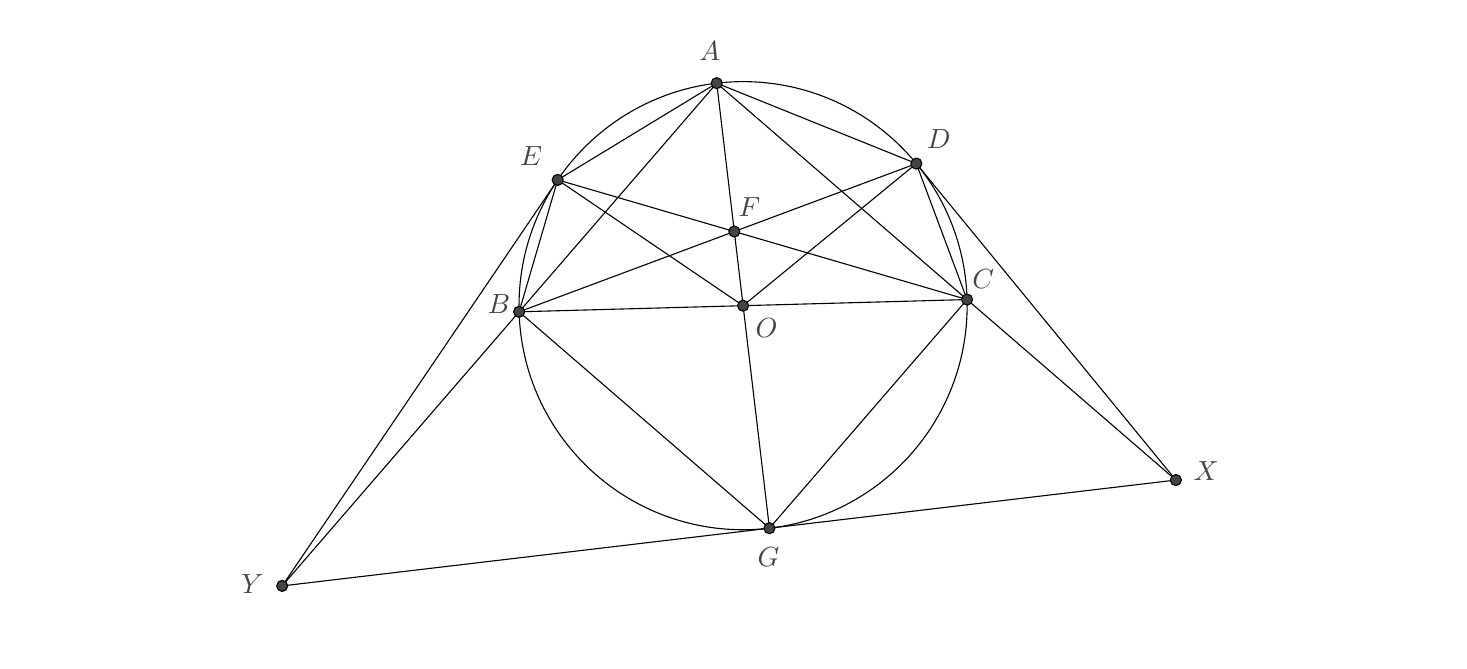
\begin{tikzpicture}[line cap=round,line join=round,>=triangle 45,x=1cm,y=1cm]
	\clip(-6.085780747970854,-1.2571901801630578) rectangle (11.837171909799954,6.5308358148891);
	\draw (3,3) circle (2.84559289761466cm);
	\draw (0.155468998430527,2.9222676382375563)-- (5.844531001569472,3.0777323617624432);
	\draw (2.665269674693615,5.825836964206406)-- (0.155468998430527,2.9222676382375563);
	\draw (2.665269674693615,5.825836964206406)-- (5.844531001569472,3.0777323617624432);
	\draw (8.496315162700949,0.7855709102046177)-- (-2.8535663315057924,-0.5588624640016117);
	\draw (0.6452857174640863,4.597723250934395)-- (5.844531001569472,3.0777323617624432);
	\draw (0.6452857174640863,4.597723250934395)-- (-2.8535663315057924,-0.5588624640016117);
	\draw (5.200264279280647,4.804504375244518)-- (8.496315162700949,0.7855709102046177);
	\draw (0.155468998430527,2.9222676382375563)-- (5.200264279280647,4.804504375244518);
	\draw (0.155468998430527,2.9222676382375563)-- (-2.8535663315057924,-0.5588624640016117);
	\draw (5.844531001569472,3.0777323617624432)-- (8.496315162700949,0.7855709102046177);
	\draw (3,3)-- (0.6452857174640863,4.597723250934395);
	\draw (3,3)-- (3.3347303253063836,0.1741630357935826);
	\draw (3,3)-- (5.200264279280647,4.804504375244518);
	\draw (2.665269674693615,5.825836964206406)-- (3,3);
	\draw (0.6452857174640863,4.597723250934395)-- (2.665269674693615,5.825836964206406);
	\draw (0.155468998430527,2.9222676382375563)-- (3.3347303253063836,0.1741630357935826);
	\draw (3.3347303253063836,0.1741630357935826)-- (5.844531001569472,3.0777323617624432);
	\draw (5.200264279280647,4.804504375244518)-- (5.844531001569472,3.0777323617624432);
	\draw (5.200264279280647,4.804504375244518)-- (2.665269674693615,5.825836964206406);
	\draw (0.6452857174640863,4.597723250934395)-- (0.155468998430527,2.9222676382375563);
	\begin{scriptsize}
		\draw [fill=uuuuuu] (3,3) circle (2pt);
		\draw[color=uuuuuu] (3.297005008478954,2.7115676584698735) node {\normalsize$O$};
		\draw [fill=uuuuuu] (0.155468998430527,2.9222676382375563) circle (2pt);
		\draw[color=uuuuuu] (-0.10012224167148483,3.0194591211273574) node {\normalsize$B$};
		\draw [fill=uuuuuu] (5.844531001569472,3.0777323617624432) circle (2pt);
		\draw[color=uuuuuu] (6.050841241082852,3.3360087872941485) node {\normalsize$C$};
		\draw [fill=uuuuuu] (2.665269674693615,5.825836964206406) circle (2pt);
		\draw[color=uuuuuu] (2.5781227508304005,6.228694908620297) node {\normalsize$A$};
		\draw [fill=uuuuuu] (5.200264279280647,4.804504375244518) circle (2pt);
		\draw[color=uuuuuu] (5.48521763205455,5.120355337684328) node {\normalsize$D$};
		\draw [fill=uuuuuu] (0.6452857174640863,4.597723250934395) circle (2pt);
		\draw[color=uuuuuu] (0.3095267568288923,4.90457241236936) node {\normalsize$E$};
		\draw [fill=uuuuuu] (8.496315162700949,0.7855709102046177) circle (2pt);
		\draw[color=uuuuuu] (8.880811400501341,0.8989462749962987) node {\normalsize$X$};
		\draw [fill=uuuuuu] (-2.8535663315057924,-0.5588624640016117) circle (2pt);
		\draw[color=uuuuuu] (-3.2303164552292193,-0.5311508317825611) node {\normalsize$Y$};
		\draw [fill=uuuuuu] (3.3347303253063836,0.1741630357935826) circle (2pt);
		\draw[color=uuuuuu] (3.3235546746457465,-0.18773142586598935) node {\normalsize$G$};
		\draw [fill=uuuuuu] (2.888423224897873,3.9419456547354685) circle (2pt);
		\draw[color=uuuuuu] (3.0802636570992056,4.257223636424458) node {\normalsize$F$};
	\end{scriptsize}
\end{tikzpicture}


\textbf{\underline{Solution 1.}}

Lấy điểm $G$ là đối xứng của $A$ qua $O$, đặt $M$ là trung điểm $BC$. Tiếp tuyến tại $G$ và $D$ của $(O)$ cắt nhau tại $X'$.\\

Ta có: $\angle GOX'=\dfrac{1}{2}\angle GOD=\angle GBD=\angle AMB\quad(AC\parallel BC)$. Từ đây suy ra $\triangle GOX'\sim\triangle AMB$. \\

Mặt khác lần lượt có $O$ và $M$ là trung điểm $AG$ và $AC$. Suy ra $\triangle GAX'\sim\triangle ACB\newline\Rightarrow\angle GAX'=\angle ACB=\angle GAC$. Ta có ngay $X'\equiv X$.\\

Ta định nghĩa $Y'$ và chứng minh $Y'\equiv Y$ tương tự. Hoàn tất chứng minh.\bigskip\\

%\textbf{\underline{Solution 2.}}
%
%Kẻ $AG$ là đường kính của $(O)$.
\end{document}